\documentclass[12pt,a4paper]{article}
\usepackage[T1]{fontenc}
\usepackage[polish]{babel}
\usepackage[utf8]{inputenc}
\usepackage{lmodern}
\usepackage{graphicx}
\usepackage{wrapfig}
\usepackage{float}
\selectlanguage{polish}


\author{
  Maciej Buczyński\qquad \texttt{kadlubken5@gmail.com}
  \and
  Tomasz Szypuła\qquad \texttt{tszypula@gmail.com}
}
\title{Model Isinga na regularnych grafach przypadkowych}

\begin{document}
\maketitle
\section{Cel ćwiczenia}
Celem ćwiczenia było zapoznanie się z symulacją modelu Isinga na regularnych grafach przypadkowych.

\section{Wstęp teoretyczny}
\subsection{Regularny graf przypadkowy}
Spiny w układzie zostały połączone w tzw. regularny graf przypadkowy, gdzie reprezentowane są przez węzły grafu, a krawędzie symbolizują połączenia między nimi. Zgodnie z definicją takiego grafu, każdy węzeł ma taką samą liczbę krawędzi, które rozmieszczone są losowo.

W dalszej części będziemy oznaczać $N$ jako całkowitą liczbę węzłów(spinów) oraz $K$ jako stopień każdego węzła.

\subsection{Model Isinga}
Model Isinga opisuje układy, gdzie spiny mają do wyboru jeden z dwóch różnych stanów. Spiny te mogą następnie oddziaływać ze sobą, prowadząc do ewolucji czasowej(iteracyjnej) układu. W naszym przypadku stanami były liczby +1 i -1.

Energię dla pojedynczego spinu w modelu Isinga określa wzór:
$$ E_{i}=-s_{i}\sum_{j}s_{j}J_{ij}$$
Gdzie $s_{i}$- i-ty spin, $J_{ij}$- stała oddziaływania między spinami $i$ oraz $j$(w naszym przypadku równa 1- oddziaływanie ferromagnetyczne), a sumowanie odbywa się po wszystkich sąsiadach $s_{i}$

Z kolei magnetyzację obliczamy na podstawie wzoru:
$$ M=\frac{\sum_{i=1}^{N}s_{i}}{N} $$
 
\section{Metoda symulacji oraz temperatura krytyczna}
W celu symulacji ewolucji czasowej układu posłużyliśmy się algorytmem Metropolis:
\begin{itemize}
\item Wybranie losowego spinu $i$ ze zbioru wszystkich spinów w grafie
\item Kalkulacja różnicy energii w przypadku zmiany spinu
\item Jeśli energia zmaleje, zmiana spinu na przeciwny. Jeśli nie, zmiana spinu jedynie z pewnym prawdopodobieństwem $e^{\frac{-\Delta E}{k_{B}T}}$
\end{itemize}

Algorytm ten pozwala symulować Model Isinga. Dzięki uwzględnieniu temperatury możemy symulować m.in. przejście fazowe ferromagnetyk- paramagnetyk oraz odwrotnie.
W czasie dążącym do nieskończoności układ z $T<T_{c}$ ulegnie samoistnej magnetyzacji(stan ferromagnetyczny). Jednak dla pewnej wartości $T_c$ szumy termiczne będą tak duże, że układ nie będzie wykazywał uporządkowanej magnetyzacji, tzn. $M\approx0$(stan paramagnetyczny). Wzór teoretyczny dla temperatury krytycznej(dla regularnych grafów przypadkowych):
$$ T_{c}=\frac{2}{ln(\frac{K}{K-2})} $$
Gdzie $K$- stopień węzła(liczba sąsiadów)

\section{Wyniki}
\subsection{Ewolucja czasowa}
\paragraph{}
Na wykresie \ref{fig:czas_T2} możemy zobaczyć przykładową zależność czasową układu dla $T<T_{c}$ z magnetyzacją początkową bliską 0.
\begin{figure}[H]
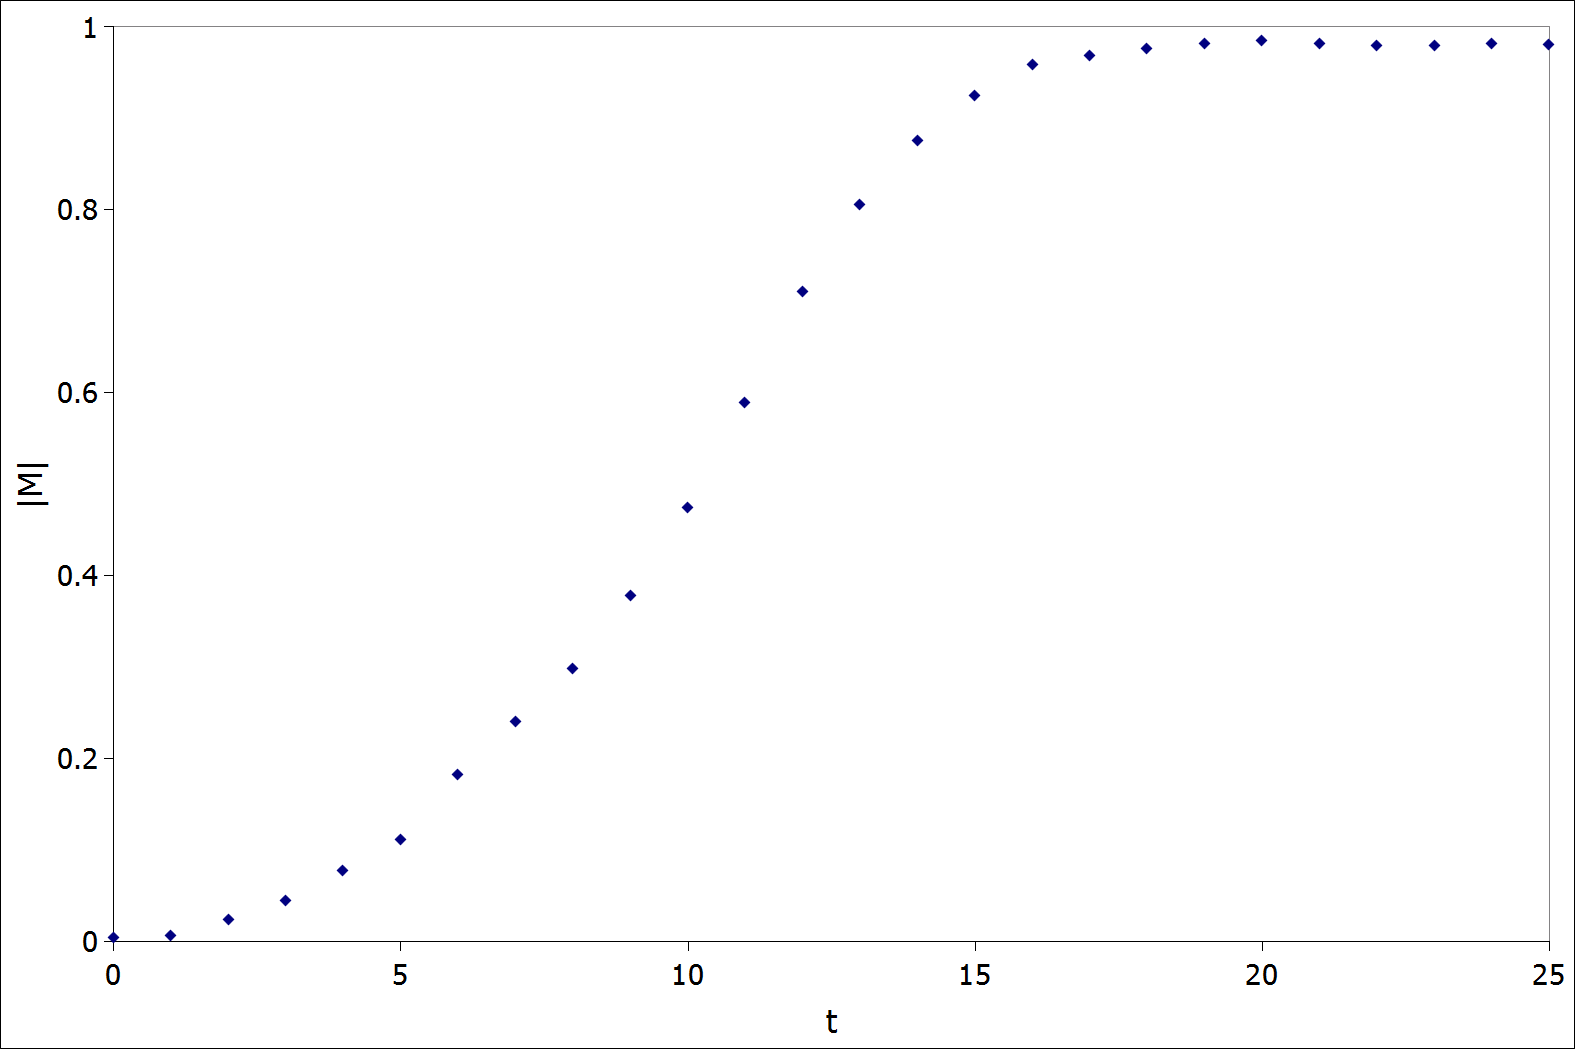
\includegraphics[width=\textwidth]{czas_T2.png}
\caption{Magnetyzacja układu dla $T=2$, $N=10000$, $K=5$}
\label{fig:czas_T2}
\end{figure}
\paragraph{}
Z kolei po zmianie temperatury powyżej $T_{c}$ układ przechodzi w stan paramagnetyczny, a jego magnetyzacja spada do 0, gdzie oscyluje potem na skutek szumów termicznych. Widać to na wykresie \ref{fig:czas_T4_5}

\begin{figure}[H]
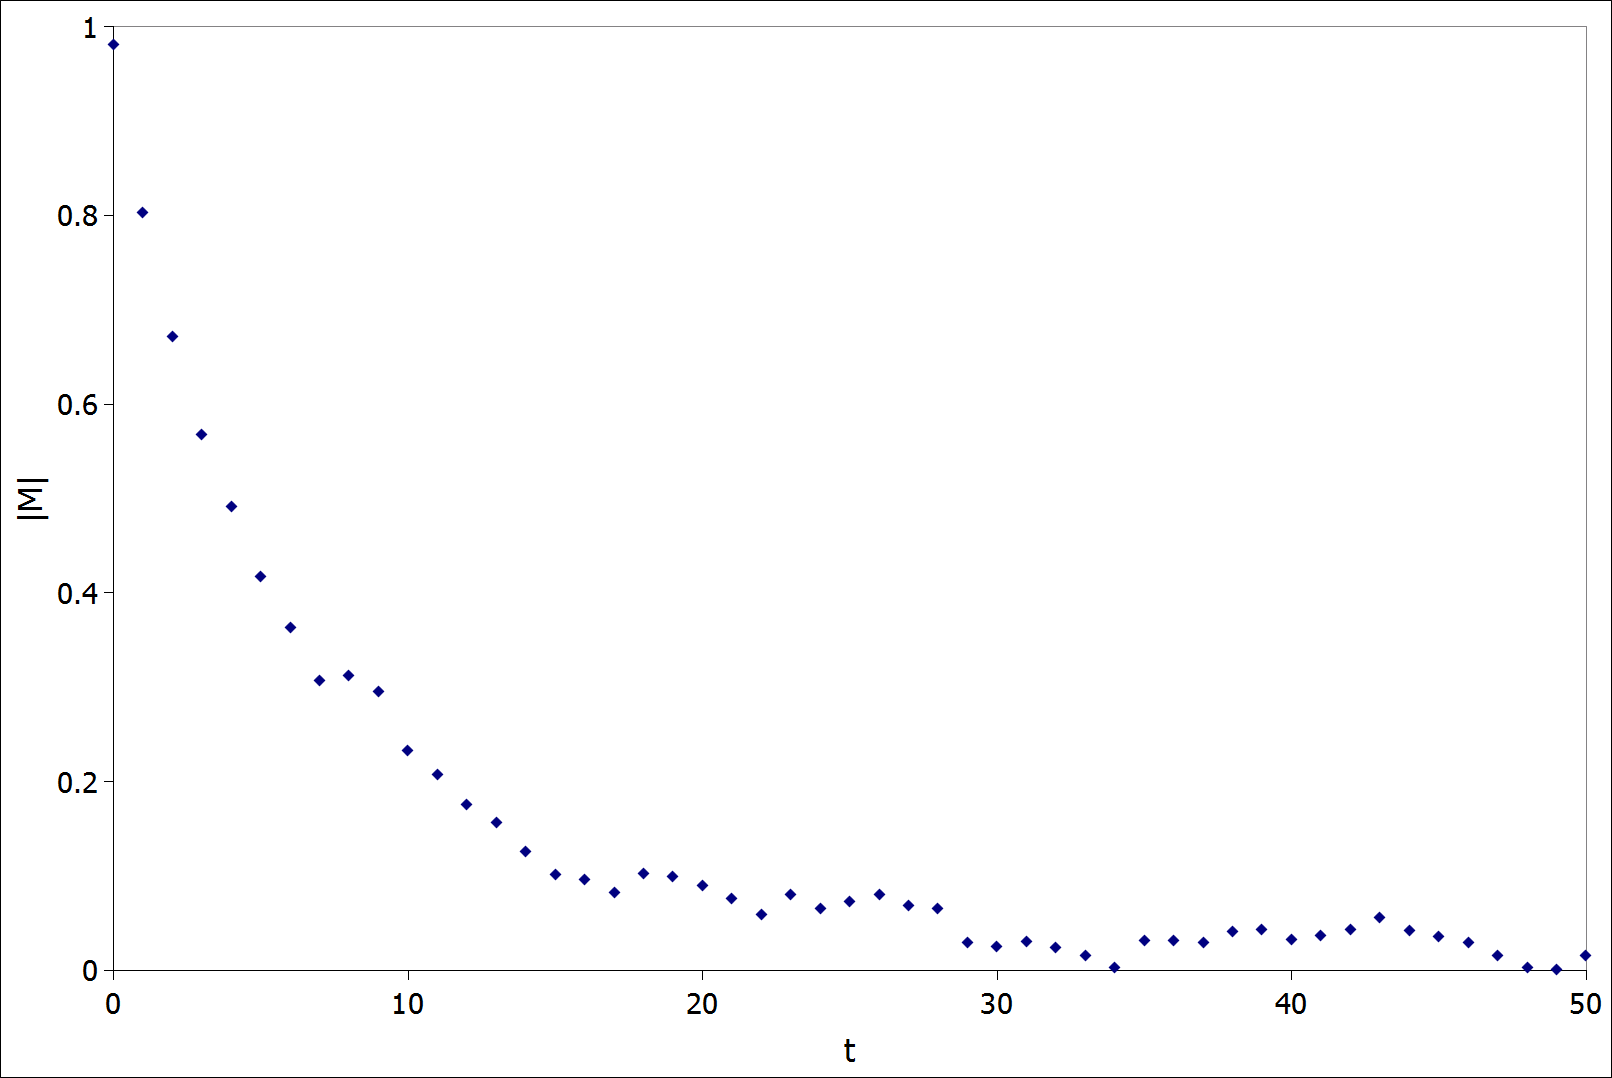
\includegraphics[width=\textwidth]{czas_T4_5.png}
\caption{Magnetyzacja układu dla $T=4.5$, $N=10000$, $K=5$}
\label{fig:czas_T4_5}
\end{figure}

\subsection{Wykresy temperaturowe}

\begin{figure}[H]
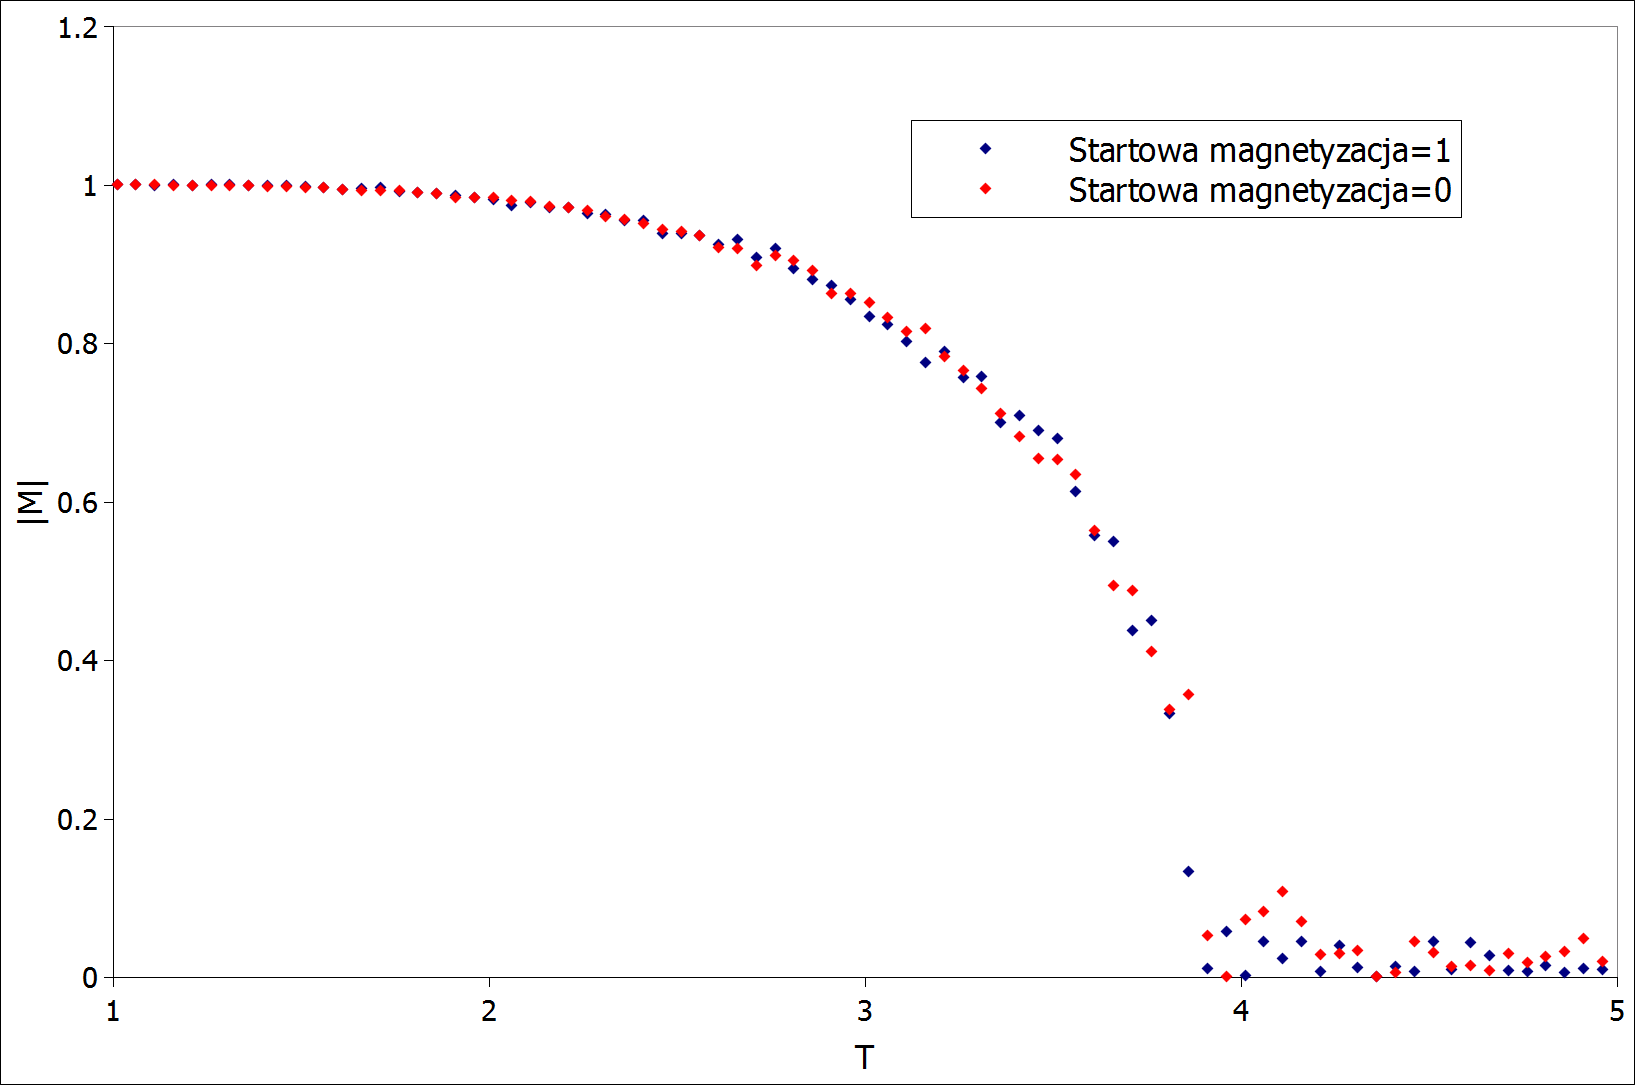
\includegraphics[width=\textwidth]{rozne_warunki_poczatkowe.png}
\caption{Porównanie spektrów temperaturowych dla różnych warunków początkowych, $N=10000$, $K=5$}
\label{fig:rozne_warunki}
\end{figure}

\paragraph{}
Na wykresie \ref{fig:rozne_warunki} można zobaczyć porównanie spektrum temperaturowego dla grafu zaczynającego się z różnym $M$. Oba zestawy danych są bardzo zbliżone, co daje podstawy do stwierdzenia, że magnetyzacja układu przy czasie dążącym do nieskończoności nie zależy od warunków początkowych. 

\begin{figure}[H]
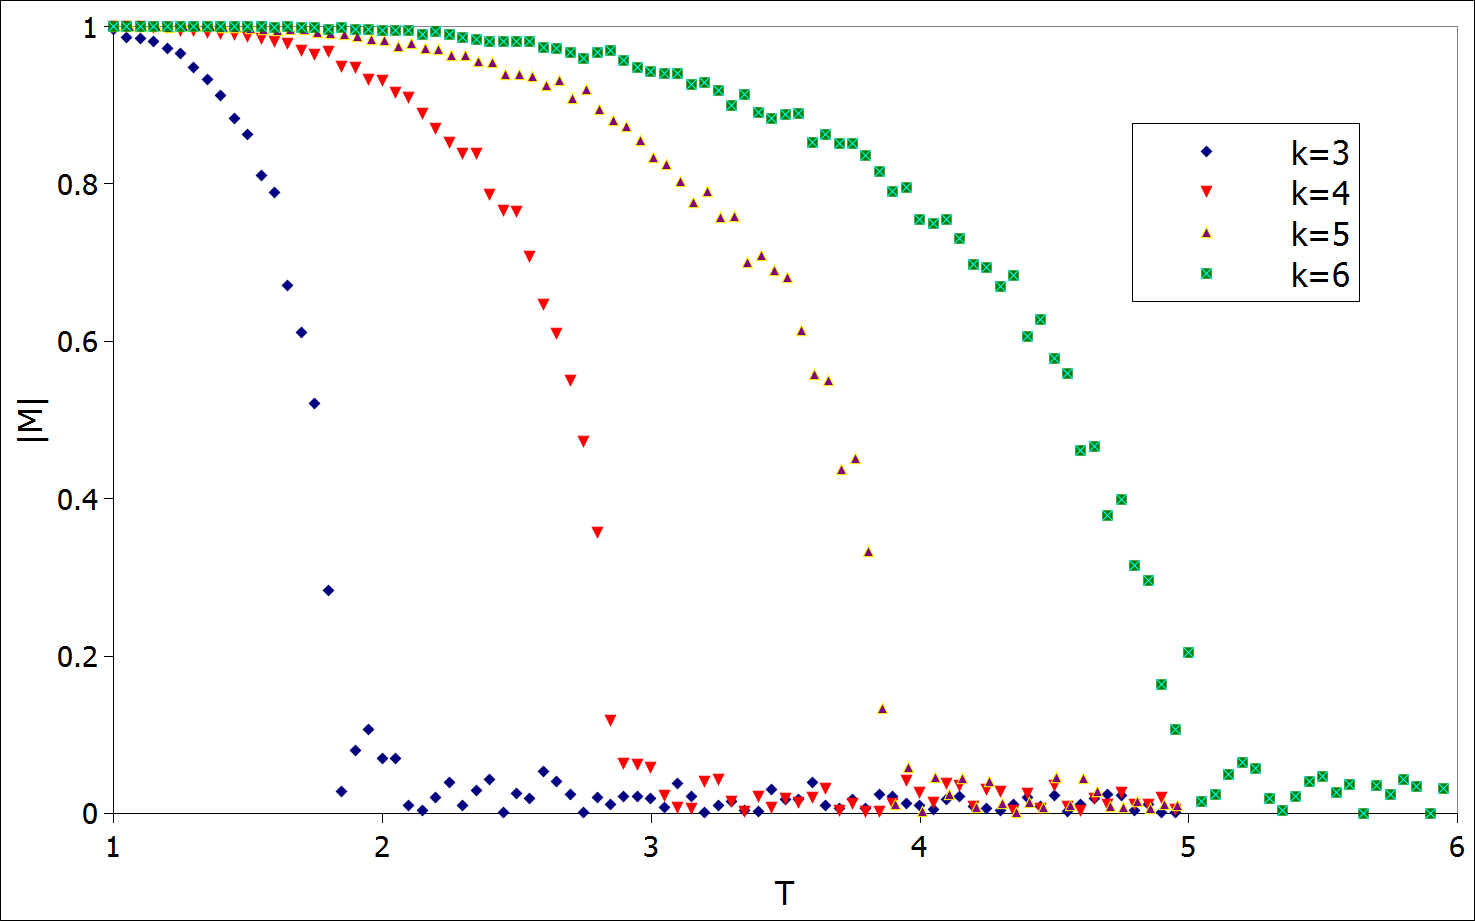
\includegraphics[width=\textwidth]{rozne_K.png}
\caption{Porównanie spektrów temperaturowych dla różnych wartości K, $N=10000$}
\label{fig:rozne_K}
\end{figure}

\paragraph{}
Na wykresie \ref{fig:rozne_K} można zobaczyć, jak zmienia się moment przejścia w stan paramagnetyczny w zależności od parametru $K$. Zgodnie ze wzorem teoretycznym większe wartości $K$ skutkują późniejszym przejściem w stan nieuporządkowany.

\paragraph{}
Na wykresach \ref{fig:TcOd1/N.1} oraz \ref{fig:TcOd1/N.2} wyraźnie widać, że wartość temperatury krytycznej bardzo szybko zbiega do teoretycznej wartości oczekiwanej. Na przykład dla grafu o stopniu węzłów równym 5, teoretyczna temperatura krytyczna wynosi około $T_{c} = 3.9152$ , już dla liczby węzłów mniejszej od $10^3$ (około 650), błąd wynosi mniej niż $2\%$.

\paragraph{}
Wykresy \ref{fig:LnTcOd1/N.1} oraz \ref{fig:LnTcOd1/N.2} powstały po zlogarytmowaniu poprzednich wykresów. Na wykresach \ref{fig:TcOd1/N.1} oraz \ref{fig:TcOd1/N.2} było widać bardzo szybkie zbieganie temperatury krytycznej, która potencjalnie mogła mieć charakter logarytmiczny. Stąd po zlogarytmowaniu chcieliśmy zobaczyć czy dane rzeczywiście będą układać się w linię prostą. Rzeczywiście powyżej pewnej wartośći krytycznej liczby węzłów , czy też, jak na wykresie, poniżej pewnej wartości krytycznej $\frac{1}{N}$, rzędu $10^-3$, temperatury krytyczne układają się w niemal poziomą linię prostą, zbiegającą do teoretycznej temperatury krytycznej.
\paragraph{}
Wykres \ref{fig:TcOdK} podsumowuje poprawne, zgodne z oczekiwaniami, zachowanie się zmiany temperatury krytycznej od stopnia węzłów, dla ustalonej liczby węzłów (w tym przypadku dla około $15 \cdot 10^3$). 
\paragraph{}
We wszystkich przypadkach już dla liczby węzłów mniejszych  od stu tysięcy, błąd wynosi dużo mniej niż ułamki procenta. Dla przykładu dla liczby węzłów około $N = 40000$ oraz stopnia węzłów $K=5$ błąd jest rzędu $10^{-6}\%$. 

\begin{figure}
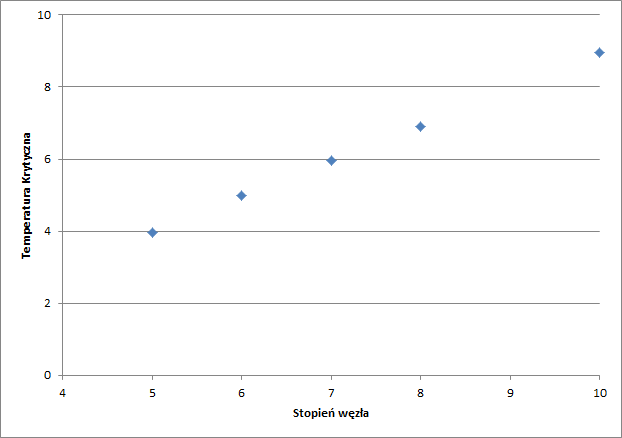
\includegraphics[width=\textwidth]{TodK.png}
\caption{Temperatura krytyczna zmierzona dla różnego stopnia węzła przy stałej liczbie węzłów}
\label{fig:TcOdK}
\end{figure}

\begin{figure}
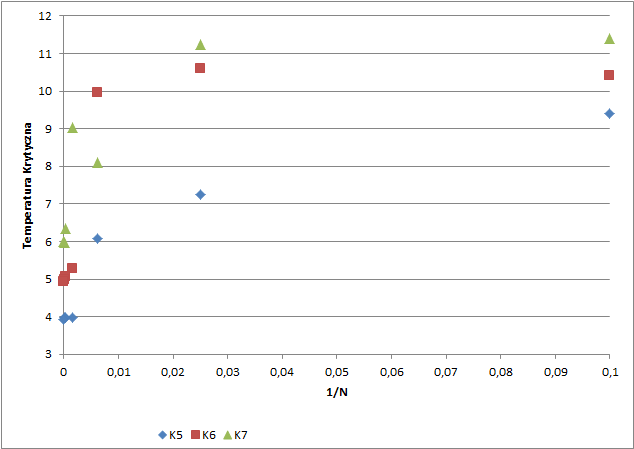
\includegraphics[width=0.8\textwidth]{K5K6K7.png}
\caption{Temperatura krytyczna w zależności od $\frac{1}{N}$, dla różnych stopni węzła}
\label{fig:TcOd1/N.1}
\end{figure}

\begin{figure}
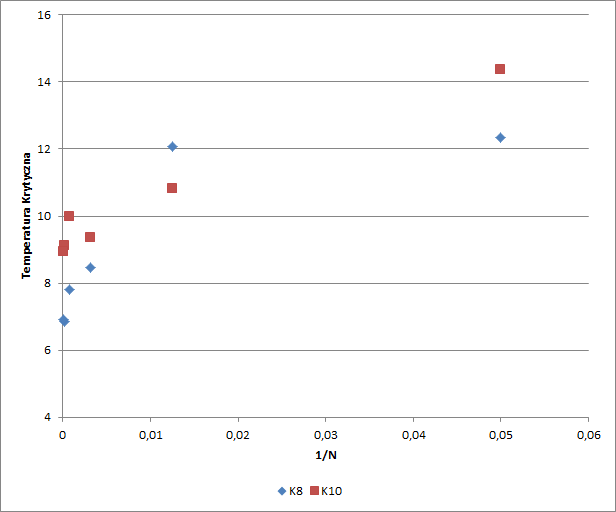
\includegraphics[width=0.8\textwidth]{K8K10.png}
\caption{Temperatura krytyczna w zależności od $\frac{1}{N}$, dla różnych stopni węzła}
\label{fig:TcOd1/N.2}
\end{figure}

\begin{figure}
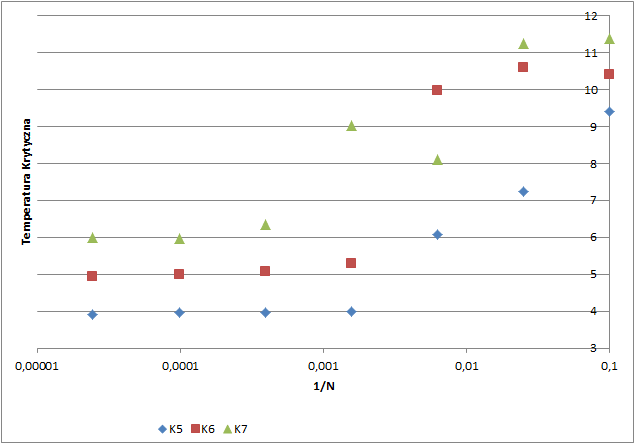
\includegraphics[width=\textwidth]{LNK5K6K7.png}
\caption{Logarytm naturalny z Temperatura krytyczna w zależności od $\ln(\frac{1}{N})$, dla różnych stopni węzła.}
\label{fig:LnTcOd1/N.1}
\end{figure}

\begin{figure}
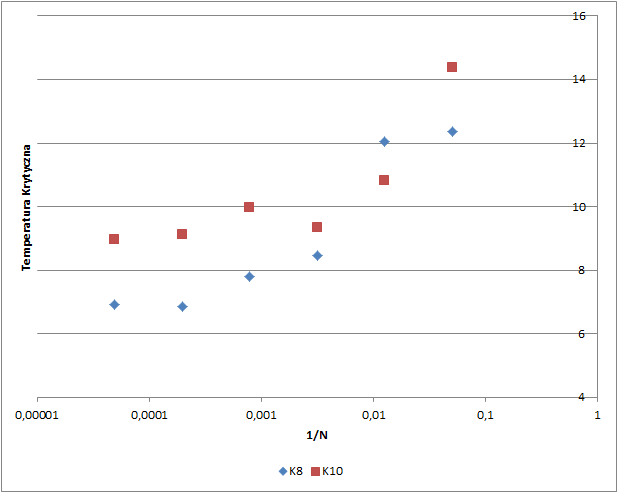
\includegraphics[width=\textwidth]{LNK8K10.png}
\caption{Logarytm naturalny z Temperatura krytyczna w zależności od $\ln(\frac{1}{N})$, dla różnych stopni węzła.}
\label{fig:LnTcOd1/N.2}
\end{figure}

\section{Wnioski}
\begin{itemize}
\item Na podstawie wykresów można stwierdzić, że wyniki zgadzają się z przewidywaniami teoretycznymi, co może świadczyć o poprawnym wykonaniu symulacji.
\item Szeregi czasowe układu są zgodne z przewidywaniami. Graf osiąga stan ferromagnetyczny dla $T<_T{c}$ oraz paramagnetyczny dla $T>T_{c}$
\end{itemize}
\end{document}